\documentclass{beamer}

% packages % 
\usepackage[utf8]{inputenc} 
\usepackage{fvextra}
\usepackage{csquotes}
\usepackage[french, italian, spanish, english]{babel}
\usepackage[T1]{fontenc} 
\usepackage{color}
\usepackage{amsmath, dsfont, amssymb, amsthm, stmaryrd}

% theme % 
\usetheme{Montpellier}
\useinnertheme{circles}
\usecolortheme{spruce}
\setbeamertemplate{itemize items}[circle]
\setbeamerfont{block title}{size=\large}
\setbeamerfont{alertblock title}{size=\large}

% images %
\usepackage{graphicx}
\graphicspath{ {./images/} }
\setbeamertemplate{caption}[numbered]

% title %
\title{Giving physical meaning to $\mathcal{W}^k(\mathfrak{g}, x, f)$}
\author{Buisine Léo \\ Supervised by UhiRinn Suh}
\institute{\textit{Ecole Normale Superieure of Paris}\\ \textit{Seoul National University}}
\date{September 2024}

% subsections intro % 
\AtBeginSection[]
{
  \begin{frame}
    \frametitle{Table of Contents}
    \tableofcontents[currentsection]
  \end{frame}
}
\setcounter{tocdepth}{1}

\begin{document}

\frame{\titlepage}

\begin{frame}
\frametitle{Table of Contents}
\tableofcontents
\end{frame}


 %% CONFORMAL FIELD THEORIES %%
\section{Introduction: CFTs and RCFTs}
\subsection{Quantum field theories}


\begin{frame}{Quantum field theories}
    \begin{figure}
      \centering
          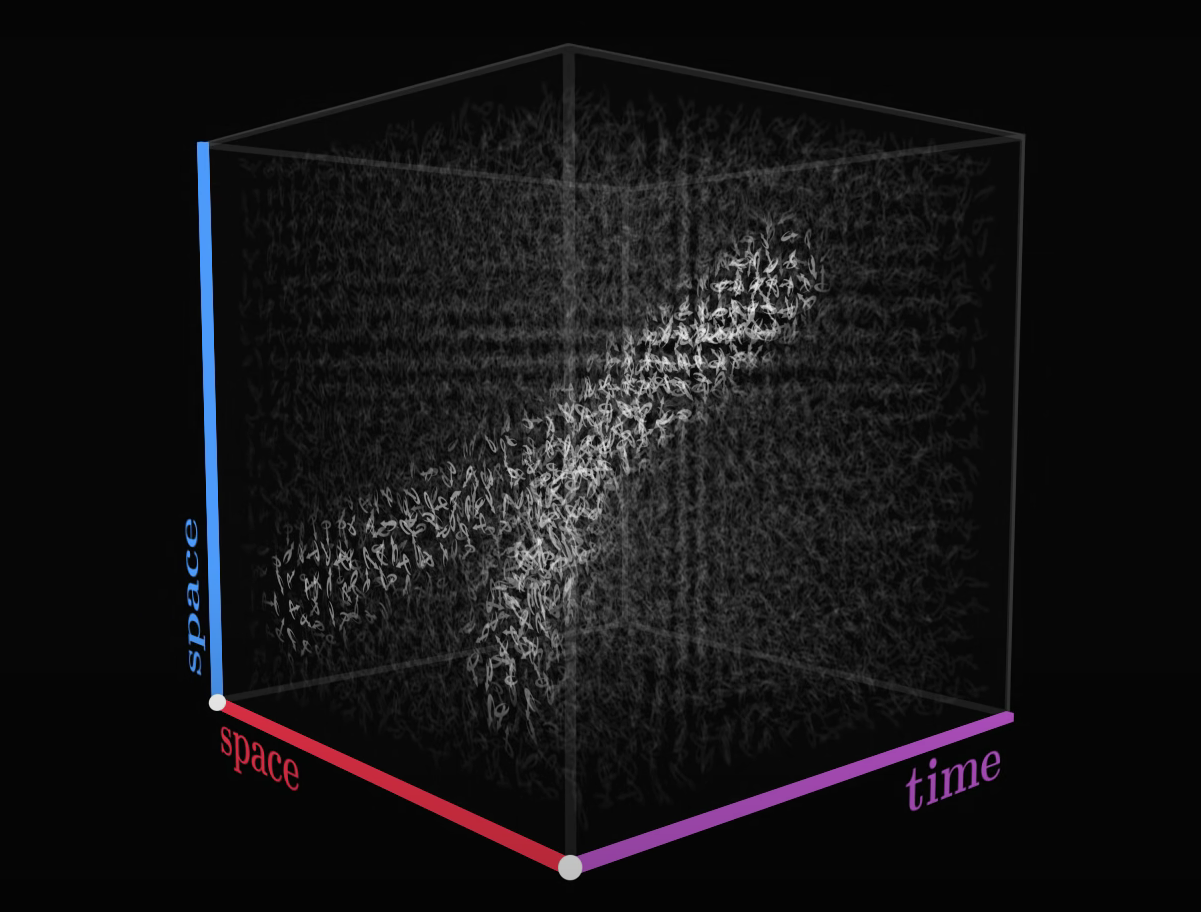
\includegraphics[width=0.7\textwidth]{qft}
          \caption{Illustration of a field}
      \end{figure}
\end{frame}


\begin{frame}{Correlation functions}
    
\end{frame}

\begin{frame}{OPE and algebra}

\end{frame}


\subsection{2D CFTs}


\begin{frame}{Conformal field theories}
    conformal symmetry
    made up of generators
\end{frame}

\begin{frame}{2D CFTs and chirality}
    in 2D, on a string, massless => left or right
\end{frame}

\begin{frame}{RCFTs}
    classification
\end{frame}

\begin{frame}{W algebras}
    general definition
\end{frame}



\section{The WZW model}
\subsection{The objective}


\begin{frame}{Objective}
    
\end{frame}


\subsection{The Sigma Model}


\begin{frame}{The Sigma model}
    
\end{frame}

\begin{frame}{Sigma model on Lie algebras}
    
\end{frame}

\begin{frame}{Conformality at two levels}
    
\end{frame}


\subsection{Adding the topological term}


\begin{frame}{Geometrical obstruction}
  \begin{block}{In CFTs}
  $[T, T] = 0$
  \end{block}
  \begin{block}{In our model}
   $[J, J] = [T, T]$ 
    \end{block}   
\end{frame}

\begin{frame}{The topological term}
    
\end{frame}

\begin{frame}{The WZW model}
    
\end{frame}


\subsection{Hypothesis}


\begin{frame}{Hypothesis: curved AKM algebras}

\end{frame}

\section{Reductions of the model}
\subsection{Reducing the model}


\begin{frame}{Toda field theory}
    
\end{frame}

\begin{frame}{Generalizing conditions}
    
\end{frame}


\subsection{Conditions}


\begin{frame}{First-classness of the conditions}
    
\end{frame}

\begin{frame}{Conformality of the reduction}
    
\end{frame}

\begin{frame}{Other conditions}
    
\end{frame}


\subsection{The algebra $\mathcal{W}(\mathfrak{g}, x, f)$}


\begin{frame}{Good gradings}
    Necessary for BRST, studied by Kac and ..
\end{frame}

\begin{frame}{$\mathcal{W}(\mathfrak{g}, x, f)$}
    
\end{frame}


\subsection{Hypothesis}


\begin{frame}{Hypothesis: relaxing the conditions}

\end{frame}



\section{Classifying through pyramids}
\subsection{Good gradings}


\begin{frame}{Good gradings}
    Necessary for BRST, studied by Kac and ..
\end{frame}


\subsection{Pyramids}


\begin{frame}{From shifting constant to blocks}
    
\end{frame}

\begin{frame}{From Hamiltonian term to pyramids}
    
\end{frame}

\begin{frame}{Reading a pyramid}
    Exemple of W(An, princip) = W(2, 3, 4, \dots)
\end{frame}


\subsection{Hypothesis}


\begin{frame}{Hypothesis: explaining infinite W algebras}
    Hypothesis about infinite W algebra, linked to infinite pyramid, nice meaning
\end{frame}

\end{document}